\newtheorem{assumption}{Assumption}
\newtheorem{hypothesis}{Hypothesis}
\newtheorem{theorem}{Theorem}
\newtheorem{defi}{Definition}
\newtheorem{prop}{Proposition}
\newtheorem{lem}{Lemma}
\newtheorem{rem}{Remark}
\newcommand{\bx}{\mathbf{x}}
\newcommand{\by}{\mathbf{y}}
\newcommand{\bu}{\mathbf{u}}
\newcommand{\bg}{\mathbf{g}}
\newcommand{\be}{\mathbf{e}}
\newcommand{\bv}{\mathbf{v}}
\newcommand{\bz}{\mathbf{z}}
\newcommand{\buu}{\mathbf{U}}
\newcommand{\bV}{\mathbf{V}}
\newcommand{\bR}{\mathbf{R}}
\newcommand{\bff}{\mathbf{f}}
\newcommand{\bX}{\mathbf{X}}
\newcommand{\bA}{\mathbf{A}}
\newcommand{\bK}{\mathbf{K}}
\newcommand{\bI}{\mathbf{I}}
\newcommand{\bE}{\mathbf{E}}
\newcommand{\bB}{\mathbf{B}}
\newcommand{\bL}{\mathbf{L}}
\newcommand{\bb}{\mathbf{b}}
\newcommand{\bc}{\mathbf{c}}
\newcommand{\bM}{\mathbf{M}}
\newcommand{\br}{\mathbf{r}}
\newcommand{\btheta}{\boldsymbol{\theta}}
\newcommand{\bbeta}{\boldsymbol{\beta}}
\newcommand{\bzero}{\mathbf{0}}
\newcommand{\bvarphi}{\boldsymbol{\varphi}}
\newcommand{\bPhi}{\boldsymbol{\Phi}}
\newcommand{\balpha}{\boldsymbol{\alpha}}
\newcommand{\bxi}{\boldsymbol{\xi}}
\newcommand{\bgamma}{\boldsymbol{\gamma}}
\newcommand{\btau}{\boldsymbol{\tau}}
\newcommand{\bnabla}{\boldsymbol{\nabla}}
\newcommand{\uth}{u^{\btheta}}
\newcommand{\fth}{f^{\btheta}}
\newcommand{\gth}{g^{\btheta}}
\newcommand{\vth}{v^{\btheta}}
\newcommand{\wth}{w^{\btheta}}
\newcommand{\zth}{z^{\btheta}}
\newcommand{\ba}{\mathbf{a}}
\newcommand{\bw}{\mathbf{w}}
\newcommand{\etk}{\eta^k}
\newcommand{\xik}{\xi^k}
\newcommand{\bbth}{{\mathbf{b}}^{\theta_3}}
\newcommand{\xiav}{\langle \bxi \rangle}
\newcommand*{\Scale}[2][4]{\scalebox{#1}{$#2$}}%
\reversemarginpar

\subsection{Poisson model problem}

Solving a 2D and 3D Poisson equation in C++, using the Trilinos set of libraries.


We seek to solve the Poisson equation
\begin{eqnarray}
-\Delta u &=& f \mbox{ in } D,\label{eq:1}\\[1ex]
%
u &=& 0 \mbox{ on } \partial D,\label{eq:2}
\end{eqnarray}

\begin{itemize}

\item In 2D:\\
$D=[0,1]^2$,   $f(x,y)=2(x(1-x)+y(1-y))$ is the source term and $u(x,y)$ is the solution to be computed.\par
We consider a finite difference (FD) scheme for solving (\ref{eq:1}). The spatial domain $D$ is discretized using a regular grid made of $(N+1)^2$ points $\bx_{ij}=(ih,jh)$ with $0\leq i,j \leq N$, $h=\frac{1}{N}$. We denote by $u_{ij}$ and $f_{ij}$ the approximate solution $u(\bx_{ij})$ and $f(\bx_{ij})$, respectively.\\
Using the centered FD scheme in 2D:
$$
-\frac{u_{i+1,j}+u_{i-1,j}+u_{i,j+1}+u_{i,j-1}-4 u_{ij}}{h^2}=f_{ij},
$$
written at each interior node $\bx_{ijk}$, $1 \leq i,j,k \leq N-1$, and taking into account the boundary conditions (\ref{eq:2}), write down a linear system \begin{equation}\label{eq:linsyst1} \bA \bu = \bb
\end{equation} of size $(N-1)^2\times (N-1)^2$, where $\bu$ is a vector that contains the $u_{ij}$ corresponding to the interior nodes.

\item In 3D: \\
$D=[0,1]^3$, $f(x,y,z)=3(x(1-x)+y(1-y)+z(1-z))$ is the source term and $u(x,y,z)$ is the solution to be computed. We consider a finite difference (FD) scheme for solving (\ref{eq:1}). The spatial domain $D$ is discretized using a regular grid made of $(N+1)^2$ points $\bx_{ij}=(ih,jh)$ with $0\leq i,j \leq N$, $h=\frac{1}{N}$. We denote by $u_{ij}$ and $f_{ij}$ the approximate solution $u(\bx_{ij})$ and $f(\bx_{ij})$, respectively. \\
Using the centered FD scheme in 3D:

$$
\Scale[1]{-\frac{u_{i+1,j,k-1}+u_{i-1,j,k-1}+u_{i,j+1,k-1}+u_{i,j-1,k-1} + u_{i+1,j,k+1}+u_{i-1,j,k+1}+u_{i,j+1,k+1}+u_{i,j-1,k+1}-6 u_{ijk}}{h^2}=f_{ijk},}
$$

written at each interior node $\bx_{ijk}$, $1 \leq i,j,k \leq N-1$, and taking into account the boundary conditions (\ref{eq:2}), write down a linear system \begin{equation}\label{eq:linsyst2} \bA \bu = \bb
\end{equation} of size $(N-1)^3\times (N-1)^3$, where $\bu$ is a vector that contains the $u_{ij}$ corresponding to the interior nodes.

\end{itemize}

\begin{figure}[t!]
  \centering
   \subfigure[2D case on N$^2$ $= 500^2$]
   {\label{fig:Poisson 2D}	   
   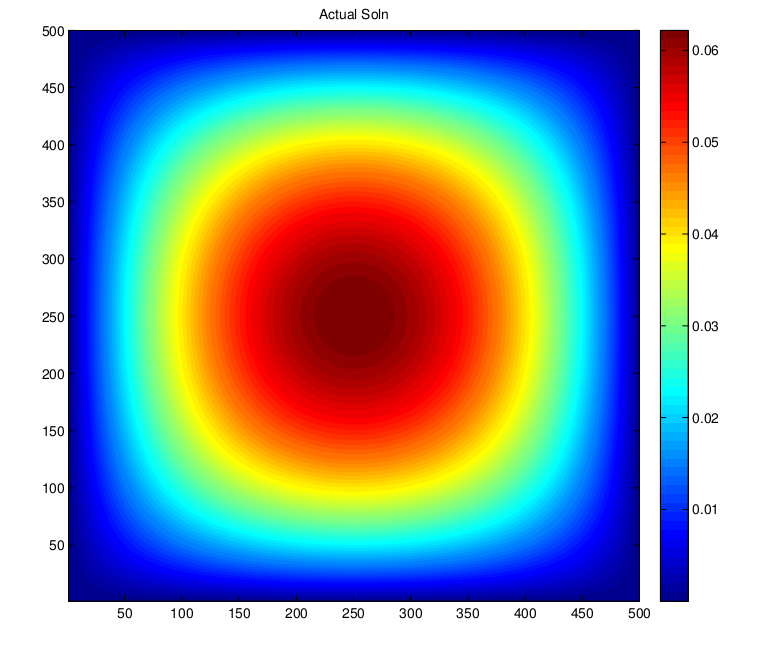
\includegraphics[height=0.35\textwidth, trim=0.2cm 0.2cm 0.2cm .2cm,clip=true]{figs/Poisson2D.png}}%
     %% 
	\:
	\subfigure[3D case on N$^3$ $= 100^3$]
   {\label{fig:Poisson 3D}	   
   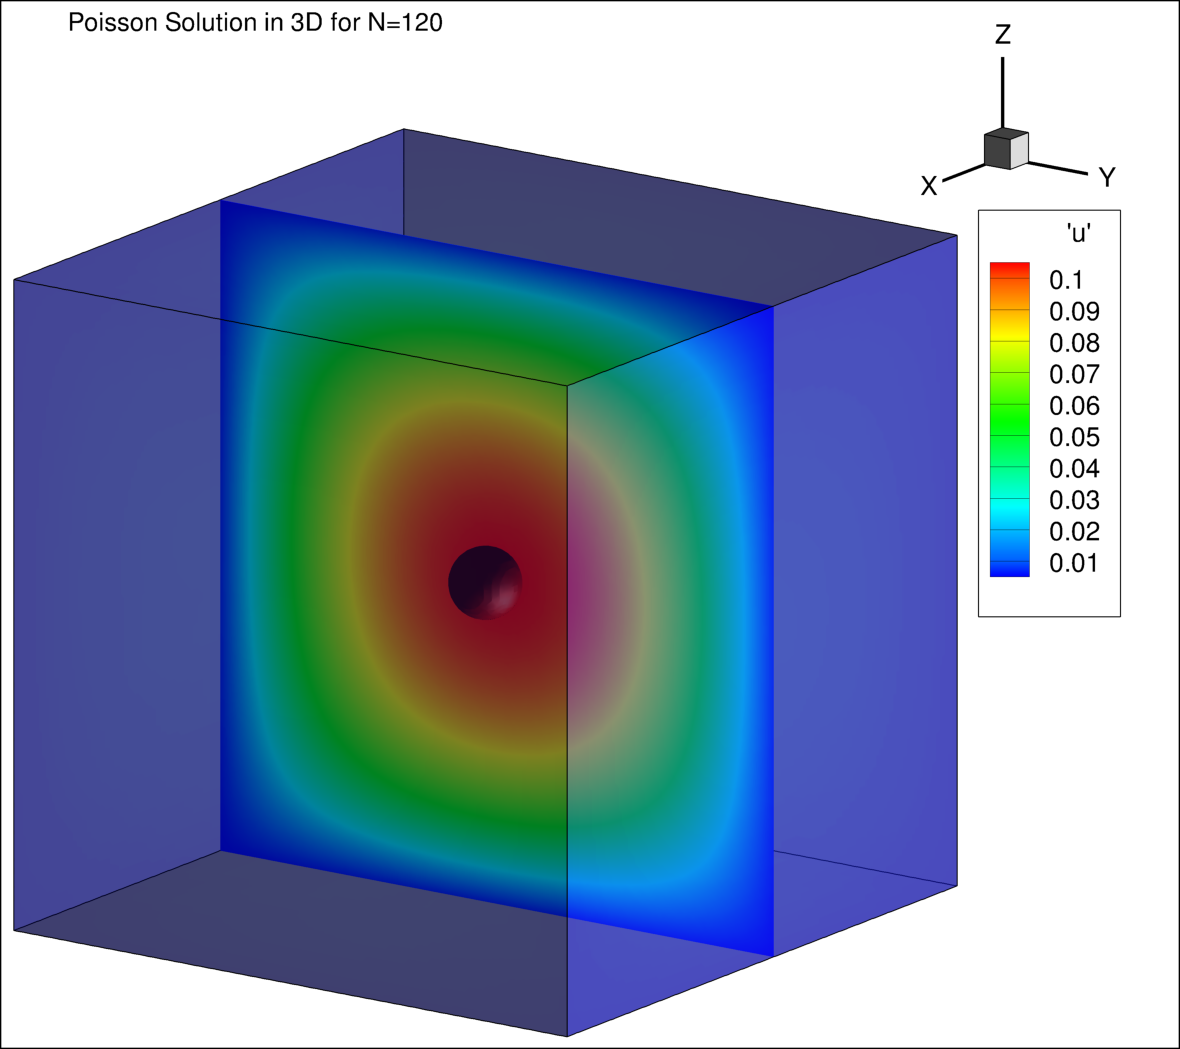
\includegraphics[height=0.35\textwidth, trim=0.2cm 0.2cm 0.2cm .2cm,clip=true]{figs/3D_Poisson.png}}%
     %%\caption{Solution Contours for the 3D solution of the Poisson Problem}  
     
    \caption{Solution Contours for solution of the Poisson Problem}  
\end{figure}